\documentclass[12pt]{article}

\usepackage[utf8]{inputenc} % declare encoding as utf8
\usepackage{graphicx} % to enable \includegraphics
\usepackage{flafter} % to make sure floats appear after their position in text
\usepackage{pdflscape} % allow some pages to be in landscape orientation
\usepackage{layout} % for debugging purposes, looking at page layout
\usepackage[margin=1in]{geometry} % leaves more space for text body
\usepackage[hidelinks]{hyperref} % hyperlinks from list of figures/tables
\usepackage[labelfont=bf]{caption} % format captions and make links go to figure instead of caption
\usepackage{csvsimple} % read and display csv files as tables
\usepackage{booktabs} % prettier tables
\usepackage{threeparttable} % easy addition of footnotes below tables
\usepackage{textcomp} % makes the \textdegree command available
\usepackage{natbib} % bibliography commands
\usepackage{tocloft} % formatting the lists of tables and figures
\usepackage{xcolor} % enable text coloring

% Formatting the table of contents/subsection
\renewcommand{\contentsname}{Supplemental methods}

% Formatting the list of tables
\renewcommand{\listtablename}{Supplemental tables} % Write "Supplemental tables" instead of "List of tables"
\renewcommand\cfttabpresnum{Table } % Write "Table" before table number in list of tables
\setlength{\cfttabnumwidth}{6em} % Spacing before captions
\setlength{\cftbeforefigskip}{1ex} % Vertical spacing between entries

% Formatting the list of figures
\renewcommand{\listfigurename}{Supplemental figures} % Write "Supplemental figures" instead of "List of figures"
\renewcommand\cftfigpresnum{Figure } % Write "Figure" before fig number in list of figures
\setlength{\cftfignumwidth}{6em} % Spacing before captions
\setlength{\cftbeforetabskip}{1ex} % Vertical spacing between entries

\graphicspath{ {figures/} } % tell Latex to look for figures in figures/

% Format figure and table numbers to follow S1, S2, ...
\renewcommand\thefigure{S\arabic{figure}} 
\renewcommand\thetable{S\arabic{table}} 

% Defining new environments as I will always want the figures centered
\newenvironment{cfigure}
	{\begin{figure} \centering}
	{\end{figure}}

\newenvironment{lsfigure}
	{\begin{landscape} \begin{figure} \centering}
	{\end{figure} \end{landscape}}

\setcounter{totalnumber}{1} % Allow a maximum of one float (table/figure) per page

\setlength{\parskip}{2ex}

% Information for the title page
\title{Supplemental data to ``Oxford Nanopore sequencing enhances structural variation discovery and genotyping from Illumina data in a Canadian soybean panel''}
\author{Marc-André Lemay \and Jonas Andreas Sibbesen \and Davoud Torkamaneh \and Jérémie Hamel \and Roger Lévesque \and François Belzile}
\date{}

% END OF PREAMBLE

\begin{document}

\maketitle \thispagestyle{empty}

\tableofcontents

\vspace{4ex}

\listoftables

\thispagestyle{empty}
\clearpage

\listoffigures

\thispagestyle{empty}

\clearpage

\section{Description and testing of the SV refinement pipeline}

One of the main objectives of this project is to use Illumina data to genotype SVs that were originally discovered using Oxford Nanopore sequencing data. 
This would enable the use Illumina data to carry out population-scale genotyping of variants that were initially discovered in a smaller set of samples sequenced with long-read technologies.

Oxford Nanopore data, however, has a high error rate.
This makes it challenging to accurately describe breakpoints and sequence content (for insertions) and may negatively impact our ability to genotype the variants discovered with this technology using short reads.

In order to address this issue, we assembled a pipeline that can be used to refine the SVs discovered by Sniffles.
By refinement, we mean that the position of the breakpoints (start and end position for deletions, and single location for insertions) and the sequence content (for insertions) can be updated to improve the quality of the variants. The current version of the pipeline ignores SVs other than deletions or insertions due to their high complexity.

The pipeline is based purely on Oxford Nanopore data (i.e. it does not need Illumina data e.g. for polishing or error correction) and therefore could potentially be used for SV refinement with any Oxford Nanopore or even PacBio dataset.

\subsection{Details of the steps in the pipeline}

The pipeline performs a local assembly of the Oxford Nanopore reads aligned to the region of interest and then uses AGE \citep{age} to align this assembly to the appropriate region of the reference genome.
This alignment is then used to update the breakpoints and inserted sequence of the variant if certain quality thresholds are met.

This alignment pipeline is largely inspired by the guidelines suggested by the authors of AGE and wtdbg2 \citep{wtdbg2} and consists of the following steps:

\begin{itemize}
	\item For every insertion or deletion, Oxford Nanopore reads overlapping the region of interest are extracted from the NGMLR \citep{ngmlr} BAM file. 
		The region of interest is a window spanning ± 200 nucleotides from the SV breakpoints (start and end of the deletion for deletions, and single location for insertions).
\item  The reads extracted in this way are assembled using wtdbg2. 
	We use preset values for Oxford Nanopore sequencing (\texttt{-x ont}) except for the following parameters: \texttt{-S 1} (no subsampling of reads), \texttt{-e} 2 (minimum read coverage of 2 for an edge in the graph), \texttt{-L 1000} (minimum read size of 1 kb), \texttt{-g 500000} (expected genome size of 500 kb).
\item A consensus sequence for the assembly is produced using the \texttt{wtpoa-cns} command from wtdbg2 with default parameters.
\item This assembly is polished using Oxford Nanopore data. For this, the same reads that were used for assembly are aligned to the consensus sequence using minimap2 \citep{minimap2} with options \texttt{-ax map-ont -r2k}. These aligned reads are used to update the consensus sequence with \texttt{wtpoa-cns}.
\item Following assembly and polishing, the reference sequence is extracted ± 500 nucleotides from the SV breakpoints for the assembled contig to be aligned against it.
\item The largest of the assembled contigs (there is usually only one) is then aligned to the reference sequence using AGE with parameters \texttt{-allpos, -go=-1} (gap opening penalty of -1 to account for the high indel error rate of Oxford Nanopore data), \texttt{-indel} (the expected excised region is an indel) and \texttt{-both} (try alignment of both the sequence and its reverse complement, and report the best alignment).
\end{itemize}

Once the alignment is completed, the results are parsed and used to extract the location of the regions excised by AGE from both the assembled contig and the reference genome.
In the case of a deletion, we expect a fragment of the reference genome to be excised, whereas in the case of a insertion, we expect a fragment of the assembled contig to be excised.
From this information, the location of the excised fragment is transformed to reference-based coordinates and the inserted sequence is extracted from the assembled contig (using the reverse complement if applicable).
The following metrics are then computed in order to compare the (refined) deletion/insertion suggested by the AGE alignment to the original (raw) one defined by Sniffles:

\begin{itemize}
	\item For deletions, the reciprocal overlap between the raw deletion and its refined counterpart. The reciprocal overlap is the minimum of the two following values: proportion of deletion 1 covered by deletion 2, and proportion of deletion 2 covered by deletion 1. This overlap is computed using functions from the GenomicRanges R package \citep{granges}.
	\item For insertions, the offset of the two insertions, i.e. the (absolute) distance between the positions of the raw and refined insertion.
	\item For insertions, the Levenshtein (edit) distance between the two inserted sequences, as computed by the R function \texttt{adist}. From this distance, a {\em distance ratio} is computed, which corresponds to the Levensthein distance between the two insertions divided by the length of the longest insertion. This provides a relative measure of the difference in sequence content between the two insertions.
\end{itemize}

In addition to the metrics related to the excised fragments themselves, the percentage of nucleotides that share identity and the percentage of nucleotides affected by gaps in the aligned regions are also extracted from the output of AGE.

Note that SVs longer than 50 kb are excluded from the pipeline because of the high memory and computing time requirements of aligning to those variants using AGE.
Although a new version of AGE called LongAGE \citep{longage} requiring less memory has been recently released, we found it unsuitable for our needs due to cryptic error messages and slower speed.

\subsection{Parameters determining whether SVs are updated or not}

Our objective is to update the position of the breakpoints and the sequence content such that the SVs updated in this way are closer to the real ones, and thus both easier to genotype from Illumina data and more representative of reality.
However, we must also avoid updating the variant in a way that is irrelevant (as would occur if, for example, AGE identified a deletion or insertion different from the target one).
Therefore, we established conditions to decide whether or not an SV should be updated.
Based on analyses carried out during the development of the pipeline, we have settled on the following thresholds to decide whether a variant should be updated:

\begin{itemize}
\item Percent identity of the alignment $\geq$ 85
\item Percentage of gaps in the assembly $\leq$ 15
\item Reciprocal overlap $\geq$ 0.5 (for deletions)
\item Edit distance ratio $\leq$ 0.5 (for insertions)
\item Offset $\leq$ 50 (for insertions)
\end{itemize}

\subsection{Testing the effect of refined SVs on genotyping performance}

The main objective of the SV refinement pipeline described above is to improve the genotyping of SVs with Illumina data.
In order to verify whether the pipeline indeed improved genotyping, we compared the genotyping precision and sensitivity of raw and refined SVs using three different genotypers: BayesTyper \citep{bayestyper}, vg \citep{vg} and Paragraph \citep{paragraph}.

\subsubsection{Application of the pipeline}

For these testing purposes, we applied the SV refinement pipeline described above to the first four samples for which we obtained Oxford Nanopore data.
Structural variants discovered using Sniffles were filtered as described in the main text (notably, only SVs genotyped as homozygous were kept) and then used as input to the pipeline.
Insertions and deletions were refined if they met the required thresholds, which were as described above except for the minimum reciprocal overlap which was set to 0.7 and the maximum distance ratio which was set to 0.45.

Table \ref{table_s4} shows the number of variants that could be refined or not for each sample.
For all four samples, a majority of SVs subjected to the pipeline met the conditions for refinement.

There can be three main reasons why a variant is not refined:

\begin{itemize}
	\item The proposed refined variant did not meet one or several quality thresholds when compared to the raw variant.
	\item The size of the variant was $>$ 50 kb.
	\item No assembly or alignment was produced by the pipeline.
\end{itemize}

In either of these cases, we simply keep the original representation of the SV as called by Sniffles.

\subsubsection{Input SV datasets}

In order to assess the effect of refining SVs on genotpying performance, we generated an input dataset of raw variants and another input dataset of refined variants.

In order to generate input datasets for genotyping, the SV sets obtained from the four samples were merged using SVmerge with parameters \texttt{-maxdist 15 -reldist 0.1 -relsizediff 0.1 -relshift 0.1 -seqspecific}.
For refined variants, the default random selection behavior of SVmerge when combining several variants together was modified to systematically favor variants that had been updated by the pipeline.

Following this, the VCF files were coordinate-sorted, normalized (using \texttt{bcftools norm}) and duplicate records were removed.

\subsubsection{Genotyping methods}

The raw and refined SV datasets were both used as input to three genotyping programs, BayesTyper, vg and Paragraph.

\paragraph{BayesTyper}

We followed the methods suggested by the authors of BayesTyper for genotyping (\url{https://github.com/bioinformatics-centre/BayesTyper}).

Briefly, k-mers were counted from the adapter-trimmed fastq files using KMC \citep{kmc} and a Bloom filter was applied using the \texttt{bayesTyperTools makeBloom} utility.

In parallel, \texttt{BayesTyperTools combine} had to be run to make the VCF input files suitable for input to BayesTyper.

Genotyping was then carried out using \texttt{bayesTyper cluster} and \texttt{bayesTyper genotype} sequentially with default parameters except for the use of the mitochondrial and chloroplastic genome sequences as decoy sequences.

Precision-recall curves for BayesTyper were generated by varying the genotype quality (GQ) threshold necessary to make a call.

\paragraph{vg}

Variation graphs were created from the VCF files using \texttt{vg construct} and then converted to PackedGraph format using \texttt{vg convert -p}. The graphs were then indexed prior to mapping using \texttt{vg index -L -x} to generate the xg index and \texttt{vg index -g} to generate the GCSA index. GCSA indexing was carried out on a version of the graph that had been pruned with \texttt{vg prune}.

Reads were mapped separately for each sample using \texttt{vg map}. These mappings were then used to call the SVs explicitly defined in the input VCF files using \texttt{vg pack -Q5} and \texttt{vg call -v}.

Precision-recall curves for vg were generated by varying the genotype quality (GQ) threshold necessary to make a call.

\paragraph{Paragraph}

VCF input files were prepared for input to Paragraph as described in the main text, i.e. variants located less than 500 nucleotides from chromosome ends were removed and variants were padded with reference nucleotides where required. Samples were genotyped separately using the \texttt{multigrmpy} utility of Paragraph.

Precision-recall curves for Paragraph were generated by varying the minimum number of reads (DP) threshold necessary to make a call.

\subsubsection{Benchmarks: raw versus realigned variants}

Benchmarks were carried out using the sveval R package \citep[][\url{https://github.com/jmonlong/sveval}]{vg} following the methods described in the main text.

\paragraph{Bayestyper}

Figure \ref{fig_s17} shows the benchmarking results obtained for BayesTyper.
Overall, the refined deletions resulted in a higher sensitivity but similar precision. 
The benefits of SV refinement were obvious for larger deletions, whereas results were sometimes worse for deletions in the range of 100-1000 nucleotides.
The improvemement brought by refinement is more obvious for insertions than it was for deletions, most likely because the refinement pipeline also improved the sequence content of the insertions.
The poor overall sensitivity of the results obtained with BayesTyper when genotyping Oxford Nanopore SVs is probably due to the small tolerance of this program to errors in SV breakpoint location or sequence content, as has been previously documented \citep{vg}.
Nevertheless, the improvement in sensitivity obtained by using refined SVs suggests that the SV refinement pipeline indeed improves the quality of the variants.

\paragraph{vg}

Figure \ref{fig_s18} shows the benchmarking results obtained for vg.
Refining the deletions does seem to have improved the results, although only very slightly.
For insertions, however, the improvement resulting from realignment is obvious, both in terms of sensitivity and precision.
Again, this suggests that the breakpoint refinement pipeline improved the accuracy of the sequence content of insertions, such that they could be more accurately genotyped by vg.

\paragraph{Paragraph}

Figure \ref{fig_s19} shows the benchmarking results obtained for Paragraph.
Using refined variants results in a slight increase in sensitivity for Paragraph, both for deletions and smaller insertions ($<$ 1,000 bp).
The apparent drop in precision for insertions $\geq$ 1,000 bp is likely due to the fact that the Oxford Nanopore data represented a poor ground truth dataset for these samples in this size range, as explained in the main text.
It is therefore expected that an increase in sensitivity from refining the variants will result in an apparent loss of precision in this size range.

\subsection{Conclusion on the SV refinement pipeline}

Overall, the results show that the breakpoint refinement pipeline results in higher genotyping sensitivity than using the raw variants as called by Sniffles.
While the results are not immediately obvious when using Paragraph, the improvements obtained using BayesTyper and vg suggest that the quality of the SVs is indeed higher following breakpoint refinement.
This is probably due to the high tolerance of Paragraph to errors in SV sequence (as documented in \cite{paragraph}) compared to the two other tools.
However, even if the improvement in genotyping performance using Paragraph is not obvious, downstream analyses should still benefit from more accurate SV breakpoints and sequence.

\subsection{Software availability}

The SV refinement pipeline described here is available from \textcolor{red}{\url{https://github.com/malemay}} (to be added later).

\clearpage

% Table S1 \caption{DNA extraction and preparation methods for Oxford Nanopore sequencing}{{{
\begin{table}
	\centering
	\caption{DNA extraction and preparation methods for Oxford Nanopore sequencing}
	\label{table_s1}

	\begin{threeparttable}\small

		\csvreader[tabular = llllcll,
		head to column names,
		table head = \toprule Sample\tnote{a} & Growth\tnote{b} & Grinding\tnote{c} & %
			     Extraction\tnote{d} & RNase T (\textdegree{}C)\tnote{e} & Size selection\tnote{f} & Combined\tnote{g} \\\midrule,
		table foot = \bottomrule]%
% DEPENDENCY : table_s1.csv
		{tables/table_s1.csv}%
		{}%
		{\sample & \growing & \grinding & \extraction & \rnase & \size & \combined}

		\begin{tablenotes}\footnotesize
		\item[a] The number in parentheses identifies samples sequenced on two different flowcells
		\item[b] Field: leaf harvested at Agriculture and Agri-Food Canada in Ottawa, and cryodessicated on site
		\item[c] Grinding method: LN + TL, Frozen in liquid nitrogen and ground using Qiagen TissueLyser;\\
			CD + TL, Cryodessicated at harvest and ground using Qiagen TissueLyser;\\
			LN + MP, Frozen in liquid nitrogen and ground using mortar and pestle
		\item[d] Extraction protocol used: CTAB, CTAB-based protocol described in main text;\\
			DNeasy, Qiagen DNeasy Plant Mini Kit;\\
			Gentra, Qiagen Gentra Puregene Tissue Kit
		\item[e] Incubation temperature of the RNase step
		\item[f] Size-selection protocol: None, no size-selection;\\
			BP 6kb, BluePippin with 6kb size-selection threshold;\\
			BP 15kb, BluePippin High-Pass Plus cassette with 15kb size-selection threshold;\\
			SRE, Circulomics Short Read Eliminator Kit
		\item[g] Indicates whether the DNA from two different extractions was combined for sequencing
		\end{tablenotes}

	\end{threeparttable}
\end{table}

\clearpage%}}}

% Table S2 \caption{Metadata on Oxford Nanopore sequencing runs}{{{
\begin{table}
	\centering

	\caption{Metadata on Oxford Nanopore sequencing runs}
	\label{table_s2}

	\begin{threeparttable}\small
		\csvreader[tabular = llccccc,
		head to column names,
		table head = \toprule Sample\tnote{a} & Date\tnote{b} & Active pores\tnote{c} &%
		Mass (ng)\tnote{d} & Run time (h)\tnote{e} & Yield (Gb)\tnote{f} & Read N50 (kb)\tnote{g} \\\midrule,
		table foot = \bottomrule]%
% DEPENDENCY : table_s2.csv
		{tables/table_s2.csv}%
		{}%
		{\sample & \date & \pores & \mass & \runtime & \yield & \nfifty}

		\begin{tablenotes}\footnotesize
		\item[a] The number in parentheses identifies samples sequenced on two different flowcells
		\item[b] Date when the sequencing run was started, format dd-mm-yyyy
		\item[c] Number of active pores on the flowcell prior to sequencing
		\item[d] Total estimated mass of the DNA library that was loaded on the flowcell
		\item[e] Duration of the sequencing run
		\item[f] Total number of bases in the fastq files following basecalling
		\item[g] Read N50 of all reads following basecalling

		\end{tablenotes}
	\end{threeparttable}
\end{table}

\clearpage%}}}

% Table S3 \caption[Number of SVs per Oxford Nanopore sample]{{{{

\begin{landscape}
\begin{table}
	\caption[Number of SVs per Oxford Nanopore sample]{
		Number of filtered variants per SV type and size class discovered by Sniffles for 17 samples subjected to Oxford Nanopore sequencing. 
		These SVs were used a a truth set for the benchmarks presented in this paper.}
	\label{table_s3}

	\begin{threeparttable}\small

		\csvreader[head to column names,
		before first line = {\begin{tabular}{lccccccccccccccccccc}%
			\toprule & \multicolumn{4}{c}{[50bp -- 100bp[} & &  \multicolumn{4}{c}{[100bp -- 1kb[} & & \multicolumn{4}{c}{[1kb -- 10kb[} & & \multicolumn{4}{c}{$\geq$ 10kb}%
			\\[0.5ex] \cmidrule{2-5} \cmidrule{7-10} \cmidrule{12-15} \cmidrule{17-20}%
			& DEL & INS & DUP & INV & & DEL & INS & DUP & INV & & DEL & INS & DUP & INV & & DEL & INS & DUP & INV %
			\\[0.5ex] \cmidrule{2-5} \cmidrule{7-10} \cmidrule{12-15} \cmidrule{17-20}},%
			late after last line = { \\ \bottomrule \end{tabular}}]%
		{tables/table_s3.csv}%
		{}%
		{\sample & \smalldel  & \smallins  & \smalldup  & \smallinv  & & %
		           \mediumdel & \mediumins & \mediumdup & \mediuminv & & %
		           \largedel  & \largeins  & \largedup  & \largeinv  & & %
			   \hugedel   & \hugeins   & \hugedup   & \hugeinv \\}

			   \begin{tablenotes}
			   \item[] DEL: deletions; INS: insertions; DUP: duplications; INV: inversions
			   \end{tablenotes}

	\end{threeparttable}

\end{table}
\end{landscape}

\clearpage%}}}

% Table S4 \caption{Classification of deletions and insertions for four samples used to test the SV refinement pipeline}{{{

\begin{table}
	\centering
	\caption{Classification of deletions and insertions for four samples used to test the SV refinement pipeline}
	\label{table_s4}

	\begin{threeparttable}\small

		\csvreader[head to column names,
		tabular = l*4{c},
		table head = {\toprule Sample & Refined\tnote{a} & Below thresholds\tnote{b} & Above max. SVLEN\tnote{c} & No alignment\tnote{d} \\\midrule},%
			table foot = {\bottomrule}]%
			% DEPENDENCY: tables/table_s4.csv
		{tables/table_s4.csv}%
		{}%
		{\sample & \refined & \belowthr & \svlen & \noalignment}

		\begin{tablenotes}\footnotesize
		\item[a] SVs that passed all filters and had their breakpoints and/or sequence content updated by the pipeline
		\item[b] Did not pass one or several thresholds applied when comparing the proposed refined SV to the raw SV
		\item[c] SV length above the maximum permissible length (50 kb used here)
		\item[d] No assembly or no alignment produced by the pipeline
		\end{tablenotes}
	\end{threeparttable}

\end{table}

\clearpage%}}}

% Table S5 \caption{Randomization test on the mean allele frequencies of SVs depending on the genic features overlapped}{{{

\begin{table}

	\centering
	\caption{Randomization test on the mean allele frequencies of SVs depending on the genic features overlapped}
	\label{table_s5}

	\begin{threeparttable}\small
		\csvreader[head to column names,
		before first line = {\begin{tabular}{l*5{c}}%
			\toprule & \multicolumn{2}{c}{Deletions} & & \multicolumn{2}{c}{Insertions} \\[0.5ex] \cmidrule{2-3} \cmidrule{5-6}%
			Genic features & Observed difference\tnote{a} & p-value\tnote{b} & & Observed difference & p-value \\\midrule},
		late after last line = {\\ \bottomrule \end{tabular}}]%
		% DEPENDENCY: tables/table_s5.csv
		{tables/table_s5.csv}%
		{}%
		{\regionfmt & \deldiff & \delp & & \insdiff & \insp \\}

		\begin{tablenotes}\footnotesize
		\item[a] Observed difference between the mean allele frequencies of the SVs overlapping the corresponding genic features
		\item[b] p-value computed from a one-sided comparison to the distribution mean differences obtained from the randomization test.
			The significance threshold was set to $\alpha = 0.05 \div 6 = 0.008$ to correct for multiple testing.
		\end{tablenotes}
	\end{threeparttable}

\end{table}

\clearpage%}}}

% Table S6 \caption{List of Gene Ontology Biological Process terms that are overrepresented ($\alpha = 0.05$) among coding sequences impacted by SVs with frequency $>$ 0.5}{{{

\begin{landscape}
\begin{table}

	\centering
	\caption{List of Gene Ontology Biological Process terms that are overrepresented ($\alpha = 0.05$) among coding sequences impacted by SVs with frequency $>$ 0.5}
	\label{table_s6}

	\begin{threeparttable}\small

		\csvreader[head to column names,
		tabular = ll*4{c},
		table head = {\toprule GO ID & Description & Number of genes\tnote{a} & Expected\tnote{b} & Observed\tnote{c} & p-value\tnote{d} \\\midrule},
		table foot = {\bottomrule}]%
		% DEPENDENCY: tables/table_s6.csv
		{tables/table_s6.csv}%
		{}%
		{\GOBPID & \Term & \Size & \ExpCount & \Count & \Pvalue}

		\begin{tablenotes}\footnotesize
		\item[a] Number of genes with corresponding GO annotation within the gene universe (whole genome except unanchored scaffolds)
		\item[b] Expected number of genes with given GO annotation within the subset of interest considering a hypergeometric distribution
		\item[c] Observed number of genes with given GO annotation within the subset of interest
		\item[d] Bonferroni-corrected p-values computed using the conditional hypergeometric test in the GOstats R package \citep{gostats}
		\end{tablenotes}
	\end{threeparttable}
\end{table}
\end{landscape}

\clearpage%}}}

% Table S7 \caption{List of Gene Ontology Biological Process terms that are underrepresented ($\alpha = 0.05$) among coding sequences impacted by SVs with frequency $>$ 0.5}{{{

\begin{landscape}
\begin{table}

	\centering
	\caption{List of Gene Ontology Biological Process terms that are underrepresented ($\alpha = 0.05$) among coding sequences impacted by SVs with frequency $>$ 0.5}
	\label{table_s7}

	\begin{threeparttable}\small

		\csvreader[head to column names,
		tabular = ll*4{c},
		table head = {\toprule GO ID & Description & Number of genes\tnote{a} & Expected\tnote{b} & Observed\tnote{c} & p-value\tnote{d} \\\midrule},
		table foot = {\bottomrule}]%
		% DEPENDENCY: tables/table_s7.csv
		{tables/table_s7.csv}%
		{}%
		{\GOBPID & \Term & \Size & \ExpCount & \Count & \Pvalue}

		\begin{tablenotes}\footnotesize
		\item[a] Number of genes with corresponding GO annotation within the gene universe (whole genome except unanchored scaffolds)
		\item[b] Expected number of genes with given GO annotation within the subset of interest considering a hypergeometric distribution
		\item[c] Observed number of genes with given GO annotation within the subset of interest
		\item[d] Bonferroni-corrected p-values computed using the conditional hypergeometric test in the GOstats R package \citep{gostats}
		\end{tablenotes}
	\end{threeparttable}
\end{table}
\end{landscape}

\clearpage%}}}

% Table S8 \caption{List of PFAM domains that are overrepresented ($\alpha = 0.05$) among coding sequences impacted by SVs with frequency $>$ 0.5}{{{

\begin{landscape}
\begin{table}

	\centering
	\caption{List of PFAM domains that are overrepresented ($\alpha = 0.05$) among coding sequences impacted by SVs with frequency $>$ 0.5}
	\label{table_s8}

	\begin{threeparttable}\small

		\csvreader[head to column names,
		tabular = ll*4{c},
		table head = {\toprule PFAM ID & Description & Number of genes\tnote{a} & Expected\tnote{b} & Observed\tnote{c} & p-value\tnote{d} \\\midrule},
		table foot = {\bottomrule}]%
		% DEPENDENCY: tables/table_s8.csv
		{tables/table_s8.csv}%
		{}%
		{\PFAMID & \Term & \Size & \ExpCount & \Count & \Pvalue}

		\begin{tablenotes}\footnotesize
		\item[a] Number of genes with corresponding PFAM annotation within the gene universe (whole genome except unanchored scaffolds)
		\item[b] Expected number of genes with given PFAM annotation within the subset of interest considering a hypergeometric distribution
		\item[c] Observed number of genes with given PFAM annotation within the subset of interest
		\item[d] Bonferroni-corrected p-values computed using the hypergeometric test in the GOstats R package \citep{gostats}
		\end{tablenotes}
	\end{threeparttable}
\end{table}
\end{landscape}

\clearpage%}}}

% Figure S1 \caption[Illumina deletion and insertion benchmarks in non-repeat regions]{{{{
\begin{cfigure}
	% DEPENDENCY : figure_s1.png
	\includegraphics[width = 5in]{figure_s1}

	\caption[Illumina deletion and insertion benchmarks in non-repeat regions]{
		Benchmarking of deletions and insertions discovered from the Illumina data in non-repeat regions. 
		Only SVs with less than 20\% overlap to regions annotated as repeats were used for these benchmarks. 
		Each line and color represents one of 17 samples. 
		Different points were obtained for a given sample by adjusting the minimum number of supporting reads required for a Paragraph call to be considered. 
		The asterisks indicate a minimum number of supporting reads of 2.
		Note that no results were available for deletions larger than 10 kb because these all overlapped repeat regions.
	}

	\label{fig_s1}

\end{cfigure}

\clearpage%}}}

% Figure S2 \caption[Illumina duplication and inversion benchmarks]{{{{
\begin{cfigure}
	% DEPENDENCY : figure_s2.png
	\includegraphics[width = 3.5in]{figure_s2}

	\caption[Illumina duplication and inversion benchmarks]{
		Benchmarking of duplications and inversions discovered from the Illumina data. 
		Each line and color represents one of 17 samples. 
		Different points were obtained for a given sample by adjusting the minimum number of supporting reads required for a Paragraph call to be considered. 
		The asterisks indicate a minimum number of supporting reads of 2.
	}

	\label{fig_s2}

\end{cfigure}

\clearpage%}}}

% Figure S3 \caption[Illumina duplication and inversion benchmarks in non-repeat regions]{{{{
\begin{cfigure}
	% DEPENDENCY : figure_s3.png
	\includegraphics[width = 3.5in]{figure_s3}

	\caption[Illumina duplication and inversion benchmarks in non-repeat regions]{
		Benchmarking of duplications and inversions discovered from the Illumina data in non-repeat regions. 
		Only SVs with less than 20\% overlap to regions annotated as repeats were used for these benchmarks. 
		Each line and color represents one of 17 samples. 
		Different points were obtained for a given sample by adjusting the minimum number of supporting reads required for a Paragraph call to be considered. 
		The asterisks indicate a minimum number of supporting reads of 2.
	}

	\label{fig_s3}

\end{cfigure}

\clearpage%}}}

% Figure S4 \caption[Relationship between Oxford Nanopore sequencing depth and genotyping precision of Illumina duplications]{{{{
\begin{cfigure}
	% DEPENDENCY : figure_s4.png
	\includegraphics[width = 4.5in]{figure_s4}

	\caption[Relationship between Oxford Nanopore sequencing depth and genotyping precision of Illumina duplications]{
		Genotyping precision of duplications discovered from Illumina data (at a minimum threshold of 2 supporting reads) for 17 samples as a function of the average Oxford Nanopore sequencing depth of that sample.
	}

	\label{fig_s4}

\end{cfigure}

\clearpage%}}}

% Figure S5 \caption[Effect of ALT allele count on genotyping performance of Illumina insertions and deletions]{{{{
\begin{cfigure}
	% DEPENDENCY : figure_s5.png
	\includegraphics[width = 5in]{figure_s5}

	\caption[Effect of ALT allele count on genotyping performance of Illumina deletions and insertions]{
		Effect of filtering variants for minimum number of ALT alleles in homozygous genotype calls (AC\_Hom) on the performance of deletion and insertion genotyping of SVs discovered from Illumina data.
		Each line and color represents a different sample.
		The curve for a given sample was obtained by varying the AC\_Hom threshold for a variant to be considered for benchmarking.
		The asterisks mark an AC\_Hom threshold of 4 ALT alleles in homozygous genotype calls in the whole population of 102 samples.
	}

	\label{fig_s5}

\end{cfigure}

\clearpage%}}}

% Figure S6 \caption[Effect of ALT allele count on genotyping performance of Illumina duplications and inversions]{{{{
\begin{cfigure}
	% DEPENDENCY : figure_s6.png
	\includegraphics[width = 3.5in]{figure_s6}

	\caption[Effect of ALT allele count on genotyping performance of Illumina duplications and inversions]{
		Effect of filtering variants for minimum number of ALT alleles in homozygous genotype calls (AC\_Hom) on the performance of duplication and inversion genotyping of SVs discovered from Illumina data.
		Each line and color represents a different sample.
		The curve for a given sample was obtained by varying the AC\_Hom threshold for a variant to be considered for benchmarking.
		The asterisks mark an AC\_Hom threshold of 6 (for duplications) or 10 (for inversions) ALT alleles in homozygous genotype calls in the whole population of 102 samples.
	}

	\label{fig_s6}

\end{cfigure}

\clearpage%}}}

% Figure S7 \caption[Effect of the number of supporting calling programs on genotyping performance of Illumina deletions and insertions]{{{{
\begin{cfigure}
	% DEPENDENCY : figure_s7.png
	\includegraphics[width = 5in]{figure_s7}

	\caption[Effect of the number of supporting calling programs on genotyping performance of Illumina deletions and insertions]{
		Effect of filtering variants for minimum number of supporting calling programs on the performance of deletion and insertion genotyping of SVs discovered from Illumina data.
		Each line and color represents a different sample.
		The curve for a given sample was obtained by varying the minimum threshold of number of supporting calling programs for a variant to be considered for benchmarking.
		The asterisks mark a minimum threshold of one supporting calling program for a variant to be considered.
		}

	\label{fig_s7}

\end{cfigure}

\clearpage%}}}

% Figure S8 \caption[Size distribution of the SVs reported by various calling programs using Illumina data]{{{{
\begin{cfigure}
	% DEPENDENCY : figure_s8.png
	\includegraphics[width = 6.5in]{figure_s8}

	\caption[Size distribution of the SVs reported by various calling programs using Illumina data]{
		Size distribution of the SVs reported by various calling programs using Illumina data.
		(A) Distribution of SV sizes in the range from -250 bp to 250 bp.
		Negative sizes represent deletions and positive sizes represent insertions.
		Duplications and inversions were omitted from this plot.
		(B) Distribution of the absolute size of deletions on a logarithmic scale.
	}

	\label{fig_s8}

\end{cfigure}

\clearpage%}}}

% Figure S9 \caption[Number of true positive and false positive deletion calls reported by various calling program combinations]{{{{
\begin{lsfigure}
	% DEPENDENCY : figure_s9.png
	\includegraphics[width = 9in]{figure_s9}

	\caption[Number of true positive and false positive deletion calls reported by various calling program combinations]{
		Number of true positive and false positive deletion genotype calls broken down by size and by the combination of tools that reported the variant for sample OAC Oxford.
		OAC Oxford was chosen as a representative sample because of its median F1 score among all 17 benchmarked samples.
		The genotype calls considered here were filtered for a minimum number of supporting reads of 2 and a minimum number of ALT alleles in homozygous genotype calls of 4 across all 102 samples in the population.
		Note the logarithmic scale on the x-axis.
	}

	\label{fig_s9}

\end{lsfigure}

\clearpage%}}}

% Figure S10 \caption[Number of true positive and false positive insertion calls reported by various calling program combinations]{{{{
\begin{cfigure}
	% DEPENDENCY : figure_s10.png
	\includegraphics[width = 6.5in]{figure_s10}

	\caption[Number of true positive and false positive insertion calls reported by various calling program combinations]{
		Number of true positive and false positive insertion genotype calls broken down by size and by the combination of tools that reported the variant for sample OAC Lakeview.
		OAC Lakeview was chosen as a representative sample because of its median F1 score among all 17 benchmarked samples.
		The genotype calls considered here were filtered for a minimum number of supporting reads of 2 and a minimum number of ALT alleles in homozygous genotype calls of 4 across all 102 samples in the population.
		Note the logarithmic scale on the x-axis.
	}

	\label{fig_s10}

\end{cfigure}

\clearpage%}}}

% Figure S11 \caption[Relationship between Oxford Nanopore read N50 and genotyping precision of Oxford Nanopore insertions]{{{{
\begin{lsfigure}
	% DEPENDENCY : figure_s11.png
	\includegraphics[width = 8in]{figure_s11}

	\caption[Relationship between Oxford Nanopore read N50 and genotyping precision of Oxford Nanopore insertions]{
		Genotyping precision of insertions discovered from Oxford Nanopore data (at a minimum threshold of 2 supporting reads) of 17 samples as a function of the read N50 of the Oxford Nanopore run(s) of that sample.
		(A) Precision of genotyping for insertions in the range 1,000 -- 10,000 bp.
		(B) Precision of genotyping for insertions $\geq$ 10,000 bp.

	}

	\label{fig_s11}
\end{lsfigure}

\clearpage%}}}

% Figure S12 \caption[Oxford Nanopore deletion and insertion benchmarks in non-repeat regions]{{{{
\begin{lsfigure}
		% DEPENDENCY : figure_s12.png
		\includegraphics[width = 9.5in]{figure_s12}

		\caption[Oxford Nanopore deletion and insertion benchmarks in non-repeat regions]{
			Benchmarking of (A) deletions and (B) insertions discovered from the Oxford Nanopore data in non-repeat regions. 
			Only SVs with less than 20\% overlap to regions annotated as repeats were used for these benchmarks. 
			Each line and color represents one of 17 samples. 
			Different points were obtained for a given sample by adjusting the minimum number of supporting reads required for a Paragraph call to be considered. 
			The asterisks indicate a minimum number of supporting reads of 2.
			Note that no results were available for deletions larger than 10 kb because these all overlapped repeat regions.
	}

		\label{fig_s12}
\end{lsfigure}

\clearpage%}}}

% Figure S13 \caption[Oxford Nanopore duplication and inversion benchmarks]{{{{
\begin{cfigure}
	% DEPENDENCY : figure_s13.png
	\includegraphics[width = 3.5in]{figure_s13}

	\caption[Oxford Nanopore duplication and inversion benchmarks]{
		Benchmarking of duplications and inversions discovered from the Oxford Nanopore data. 
		Each line and color represents one of 17 samples. 
		Different points were obtained for a given sample by adjusting the minimum number of supporting reads required for a Paragraph call to be considered. 
		The asterisks indicate a minimum number of supporting reads of 2.
	}

	\label{fig_s13}

\end{cfigure}

\clearpage%}}}

% Figure S14 \caption[Oxford Nanopore duplication and inversion benchmarks in non-repeat regions]{{{{
\begin{cfigure}
	% DEPENDENCY : figure_s14.png
	\includegraphics[width = 3.5in]{figure_s14}

	\caption[Oxford Nanopore duplication and inversion benchmarks in non-repeat regions]{
		Benchmarking of duplications and inversions discovered from the Oxford Nanopore data in non-repeat regions.
		Only SVs with less than 20\% overlap to regions annotated as repeats were used for these benchmarks. 
		Each line and color represents one of 17 samples. 
		Different points were obtained for a given sample by adjusting the minimum number of supporting reads required for a Paragraph call to be considered. 
		The asterisks indicate a minimum number of supporting reads of 2.
	}

	\label{fig_s14}

\end{cfigure}

\clearpage%}}}

% Figure S15  \caption[Joint Illumina/Oxford Nanopore deletion and insertion benchmarks]{{{{
\begin{lsfigure}
	% DEPENDENCY : figure_s15.png
	\includegraphics[width = 9.5in]{figure_s15}

	\caption[Joint Illumina/Oxford Nanopore deletion and insertion benchmarks]{
		Benchmarking of (A) deletions and (B) insertions in the merged dataset of SVs discovered from the Illumina and Oxford Nanopore data.
			Each line and color represents one of 17 samples. 
			Different points were obtained for a given sample by adjusting the minimum number of supporting reads required for a Paragraph call to be considered. 
			The asterisks indicate a minimum number of supporting reads of 2.
	}

	\label{fig_s15}
\end{lsfigure}

\clearpage%}}}

% Figure S16 \caption[Joint Illumina/Oxford Nanopore deletion and insertion benchmarks in non-repeat regions]{{{{
\begin{lsfigure}
	% DEPENDENCY : figure_s16.png
	\includegraphics[width = 9.5in]{figure_s16}

	\caption[Joint Illumina/Oxford Nanopore deletion and insertion benchmarks in non-repeat regions]{
		Benchmarking of (A) deletions and (B) insertions in non-repeat regions in the merged dataset of SVs discovered from the Illumina and Oxford Nanopore data. 
		Only SVs with less than 20\% overlap to regions annotated as repeats were used for these benchmarks. 
		Each line and color represents one of 17 samples. 
		Different points were obtained for a given sample by adjusting the minimum number of supporting reads required for a Paragraph call to be considered. 
		The asterisks indicate a minimum number of supporting reads of 2.
		Note that no results were available for deletions larger than 10 kb because these all overlapped repeat regions.
	}

	\label{fig_s16}
\end{lsfigure}

\clearpage%}}}

% Figure S17 \caption{Genotyping benchmark of raw and refined Oxford Nanopore SVs for four samples using BayesTyper}{{{
\begin{lsfigure}
	% DEPENDENCY : figure_s17.png
	\includegraphics[width = 9.5in]{figure_s17}

	\caption{Genotyping benchmark of raw and refined Oxford Nanopore SVs for four samples using BayesTyper.}

	\label{fig_s17}

\end{lsfigure}

\clearpage%}}}

% Figure S18 \caption{Genotyping benchmark of raw and refined Oxford Nanopore SVs for four samples using vg}{{{
\begin{lsfigure}
	% DEPENDENCY : figure_s18.png
	\includegraphics[width = 9.5in]{figure_s18}

	\caption{Genotyping benchmark of raw and refined Oxford Nanopore SVs for four samples using vg}

	\label{fig_s18}

\end{lsfigure}

\clearpage%}}}

% Figure S19 \caption{Genotyping benchmark of raw and refined Oxford Nanopore SVs for four samples using Paragraph}{{{
\begin{lsfigure}
	% DEPENDENCY : figure_s19.png
	\includegraphics[width = 9.5in]{figure_s19}

	\caption{Genotyping benchmark of raw and refined Oxford Nanopore SVs for four samples using Paragraph}

	\label{fig_s19}

\end{lsfigure}

\clearpage%}}}

% Figure S20 \caption[IGV screenshot of Oxford Nanopore and Illumina read alignments at the location of a polymorphic Stowaway TE insertion]{{{
\begin{lsfigure}
	% DEPENDENCY : Gm04_2257090_annotated.png
	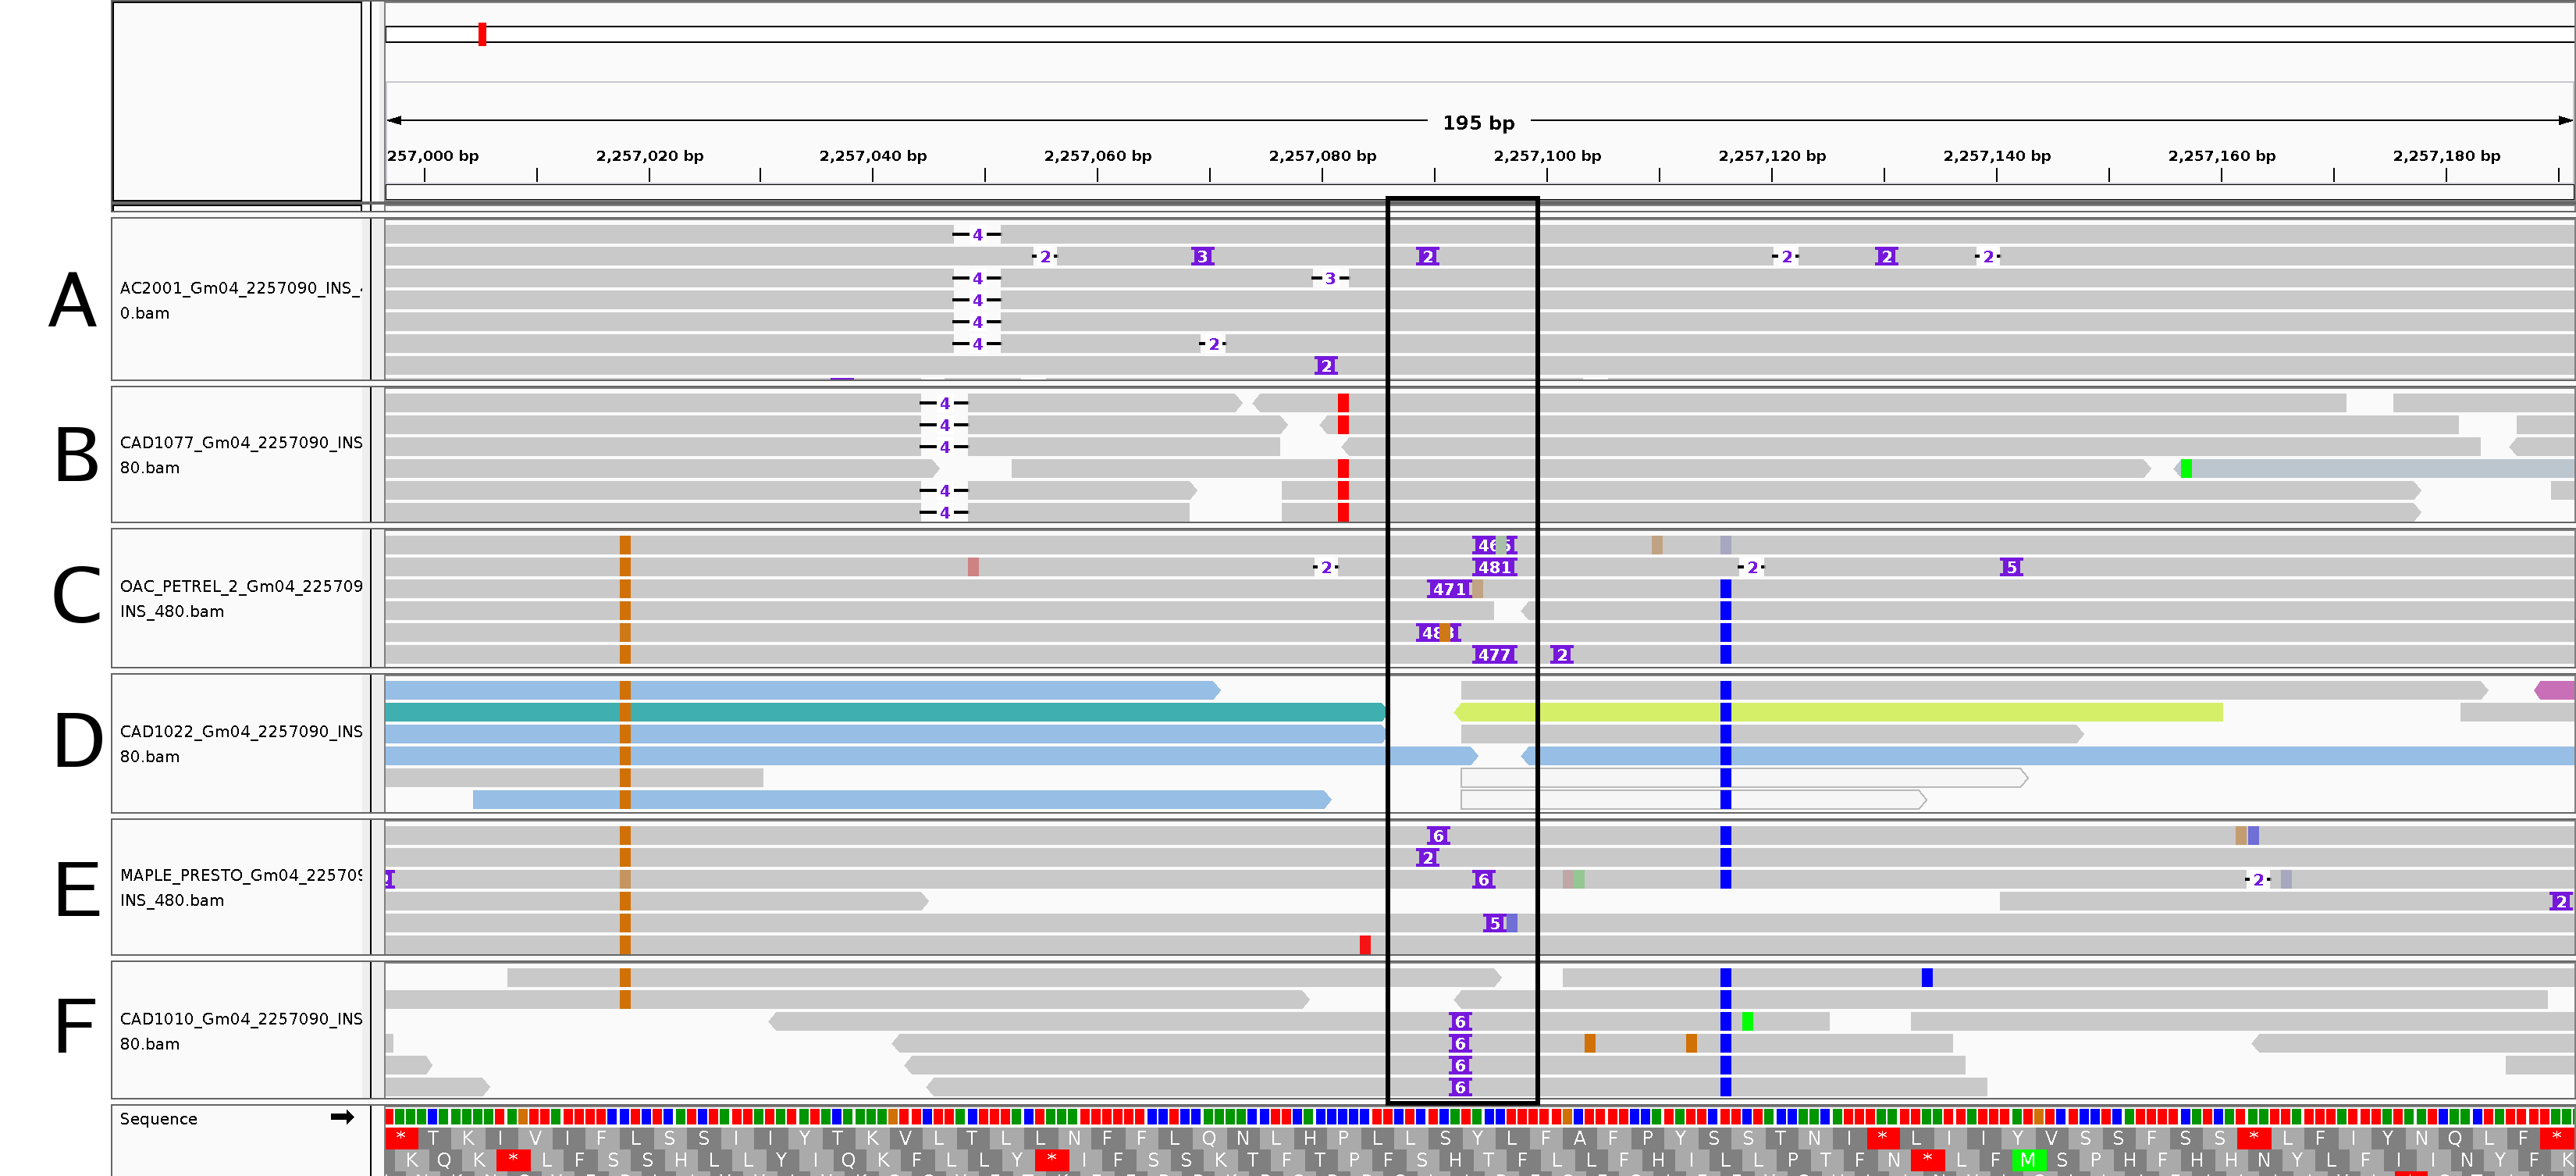
\includegraphics[width = 9.5in]{Gm04_2257090_annotated}

	\caption[IGV screenshot of Oxford Nanopore and Illumina read alignments at the location of a polymorphic Stowaway TE insertion]{
		IGV screenshot of Oxford Nanopore and Illumina read alignments at the location of a polymorphic Stowaway TE insertion at Gm04:2,257,090.
		Oxford Nanopore (A) and Illumina (B) alignments of sample CAD1077/AC2001, which matches the reference (absence of TE insertion).
		Oxford Nanopore (C) and Illumina (D) alignments of sample CAD1022/OAC Petrel, which bears the 480-bp Stowaway TE insertion.
		Oxford Nanopore (E) and Illumina (F) alignments of sample CAD1010/Maple Presto, which bears a 6-bp insertion putatively due to excision of the TE.
		The black rectangle in the middle of the figure encloses the region where the insertion polymorphisms of interest occur.
	}

	\label{fig_s20}

\end{lsfigure}

\clearpage%}}}

% Figure S21 \caption[IGV screenshot of Oxford Nanopore and Illumina read alignments at the location SNP that diverges between the Stowaway TE insertion and excision haplotypes]{{{
\begin{lsfigure}
	% DEPENDENCY : Gm04_2254504_annotated.png
	\includegraphics[width = 9.5in]{Gm04_2254504_annotated}

	\caption[IGV screenshot of Oxford Nanopore and Illumina read alignments at the location of a SNP that diverges between the Stowaway TE insertion and excision haplotypes]{
		IGV screenshot of Oxford Nanopore and Illumina read alignments at the location of a SNP (at Gm04:2,254,504) that diverges between the Stowaway TE insertion and excision haplotypes.
		Oxford Nanopore (A) and Illumina (B) alignments of sample CAD1077/AC2001, which matches the reference (absence of TE insertion).
		Oxford Nanopore (C) and Illumina (D) alignments of sample CAD1022/OAC Petrel, which bears the 480-bp Stowaway TE insertion.
		Oxford Nanopore (E) and Illumina (F) alignments of sample CAD1010/Maple Presto, which bears a 6-bp insertion putatively due to excision of the TE.
		The black rectangle in the middle of the figure encloses the SNP that diverges from the reference genome only in the haplotype that bears the Stowaway insertion.
	}

	\label{fig_s21}

\end{lsfigure}

\clearpage%}}}

% DEPENDENCY : genome_research.bst
\bibliographystyle{genome_research}
% DEPENDENCY : references.bib
\bibliography{references}

\end{document}

